% Chapter 6

\chapter{Implementación} % Main chapter title

\label{Chapter6} % Change X to a consecutive number; for referencing this chapter elsewhere, use \ref{ChapterX}

En este capítulo se explica la implementación del modelo de sistema propuesto en los capítulos anteriores, se generaron los escenarios de prueba pertinentes para los cuatro modelos que comprende nuestro simulador y se muestran resultados específicos por cada modelo. Por último, se definió la metodología en cómo se interconectaron estos cuatro modelos con el fin de dar por terminada la fase de implementación y con esto poder generar distintos resultados globales del simulador en el capítulo siguiente.

%----------------------------------------------------------------------------------------
%	SECTION 
%----------------------------------------------------------------------------------------

\section{Generación de una geometría estocastica}\label{generarGeoEstocastica}

Generación de Puntos de Poisson en un círculo: \newline

Para una generación de puntos en un círculo correcta que cumpla con la definición de un HPPP [Sección \ref{PPP_C4}], el número total de puntos que se formaron en el círculo siguió una variable aleatoria de Poisson, además, estos puntos se distribuyeron de acuerdo a una distribución uniforme dentro del círculo, por último, al considerar un proceso homogéneo, la densidad de los puntos fue constante.\newline

1. Número total de puntos:\newline

En primer lugar, para cumplir con la definición de HPPP, el número total de puntos tendrá que seguir una distribución de Poisson. Para esto en cada realización se generó una variable aleatoria de Poisson con tasa constante $\lambda$ y media $\lambda A$ donde $A=\pi r^{2}$. \newline

2. Ubicación de los puntos:\newline

Después, para la distribución uniforme de puntos en un círculo, se consideraron dos variables aleatorias uniformes, una que represente el radio y otra el ángulo (esto con base en las coordenadas polares).\newline

Entonces, debido a que el área aumenta de manera cuadrática con relación al radio, un punto aleatorio ubicado uniformemente en un círculo de radio $r$ tiene las coordenadas polares $[r(\sqrt{U}), 2\pi V]$, donde U y V son las dos variables aleatorias uniformes independientes, $U, V \in{[0,1]}$.

\subsection{Escenario de Prueba de PPP}

En este escenario se validó la generación de una geometría estocastica siguiendo un HPPP.\newline

En primer lugar, el número total de puntos debe seguir una distribución discreta de Poisson, esta se comprobó con la generación de la variable aleatoria Poisson en Python usando la libreria \textit{scipy} [Véase Apéndice~\ref{AppendixA}].\newline

Después, se comprobó la generación de puntos aleatorio ubicados uniformemente en un círculo de radio $r$ en coordenadas polares $[r(\sqrt{U}), 2\pi V]$.\newline

Se graficó en un círculo 2D la generación de puntos, con tasa constante $\lambda = 1x10_3$ y $r = 100$ con media $\lambda A$ donde $A=\pi r^{2}$ [\textit{véase Figura~\ref{fig:PPPCirculo1}}].

Por último, se validó que todos los puntos se generen dentro del areá del circulo, para esto se graficó de igual manera la distribución espacial de los puntos en un círculo en plano 2D pero ahora con una densidad mayor ($\lambda = 1x10_6$), de modo que se observe que los puntos rellenan toda el área del círculo [\textit{véase Figura~\ref{fig:PPPCirculo2}}].

\begin{figure}
    \centering
    \begin{minipage}{.45\linewidth}
      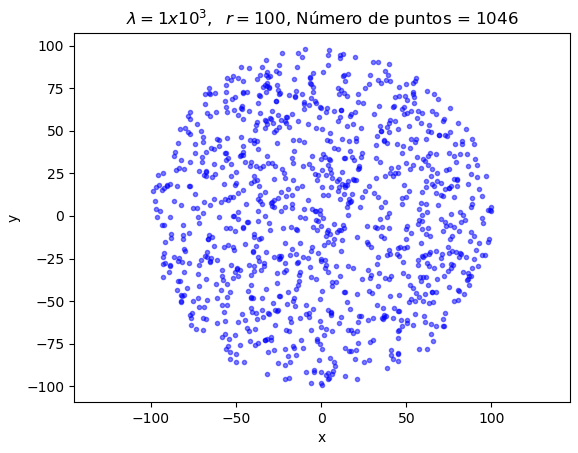
\includegraphics[width=\linewidth]{PPPCirculo1}
      \caption[Distribución espacial de puntos PPP en un círculo 2D]{Distribución espacial de puntos PPP con media $\lambda A$ en un círculo 2D}
      \label{fig:PPPCirculo1}
    \end{minipage}
    \hspace{.05\linewidth}
    \begin{minipage}{.45\linewidth}
      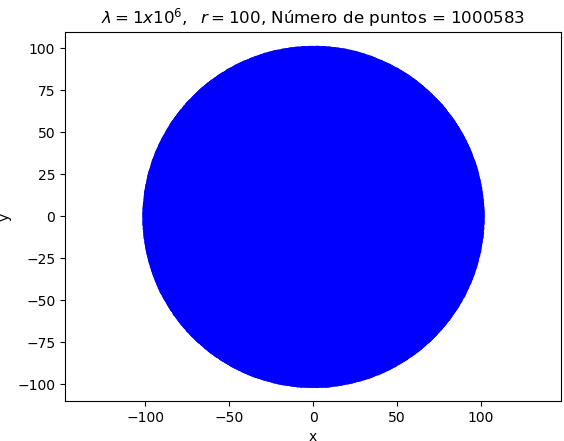
\includegraphics[width=\linewidth]{PPPCirculo2}
      \caption[Distribución espacial de puntos PPP en un círculo 2D]{Distribución espacial de puntos PPP con media $\lambda A$ en un círculo 2D}
      \label{fig:PPPCirculo2}
    \end{minipage}
\end{figure}

\break
%----------------------------------------------------------------------------------------
%	SECTION 
%----------------------------------------------------------------------------------------
\section{Generación de ganancias de canal implementando pérdidas por distancia (PLE) y desvanecimiento Rayleigh}

De acuerdo con el modelo de canal propuesto, el modelo CI (\textit{Ecuación~\ref{eqn:CI}} de \parencite{Sun2016}), este implementa pérdidas de acuerdo con la distancia y frecuencia, dado un exponente de pérdida por trayectoria (PLE) y agrega pérdidas por el desvanecimiento rápido de Rayleigh.\newline

En primera instancia, para el cálculo de la pérdida por trayectoria, se utilizó la ecuación~\ref{eqn:CI}.

Retomando lo estudiado en la Sección~\ref{DesvRayleigC2}, se tiene que cuando el desvanecimiento es tipo Rayleigh, la magnitud (amplitud) de la señal es distribuida por una variable aleatoria tipo Rayleigh pero en potencia es distribuida exponencialmente con media unitaria. \newline

La ganancia de desvanecimiento Rayleigh se modeló por medio de la generación de una variable aleatoria que siguió una distribución Rayleigh con desviación estándar unitaria, la generación de esta variable se puede ver en el Apéndice~\ref{AppendixA}.

\subsection{Escenario de Prueba de la pérdida por trayectoria}

Se propuso un escenario UMa en exteriores en un ambiente con línea de vista (LoS), entonces de acuerdo con la Tabla~\ref{tab:ModeloCI}, los parámetros válidos del modelo de canal CI en ambientes LoS, son: PLE = 2; frecuencia de operación = 2- 38GHz; rango de distancias 60- 930 m. La Figura ~\ref{fig:PerdidasCI_C6} muestra las pérdidas por trayectoria que dependen de las distancias (entre BS y UE) y frecuencias en todo el rango en el cual es válido este modelo (sin tomar en cuenta el desvanecimiento). Se observa el incremento de las pérdidas conforme aumentan la distancia y la frecuencia. \newline

\begin{figure}[th]
    \centering
    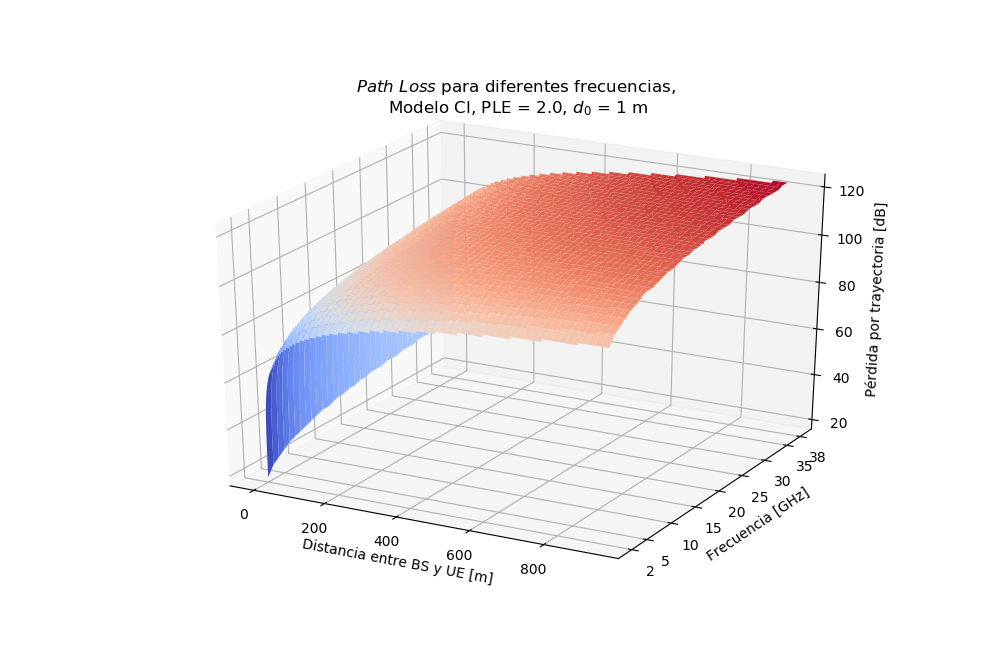
\includegraphics[scale=.6]{Figures/MODELOCI3D_1m.png}
    \decoRule
    \caption[Pérdidas por trayectoria según el Modelo CI]{Pérdidas por trayectoria según el Modelo CI}
    \label{fig:PerdidasCI_C6}
\end{figure}

\subsection{Escenario de Prueba del Modelo de canal CI}

Ahora bien, al incorporar el desvanecimiento tipo Rayleigh y las pérdidas por trayectoria, siguiendo la Tabla~\ref{tab:ParametrosGral} donde se definen los parámetros de la simulación (PLE= 2 con radio celular de 200m, en una banda de 2 GHz), se generó el histograma (pdf) de los coeficientes de canal (ganancias de canal) esperados para el simulador, véase Figura~\ref{fig:GananciasCI_C6}, se puede observar que el valor promedio de las ganancias ($h$) es de 80.35 dB. \newline

Para la generación de las ganancias $h$ se utilizó la siguiente Ecuación:\newline

\begin{equation}
    h =  10^{(\frac{-L_{p [dB]}^{CI}}{10})} \cdot \gamma\ [W]
    \label{eqn:h_canal}
\end{equation}
Donde:
\[\gamma \to ganancia\ desvanecimiento\ Rayleigh\]
\[\ L_{p [dB]}^{CI} \to \textit{Path\ Loss}\ Modelo\ CI \]

\begin{figure}[th]
    \centering
    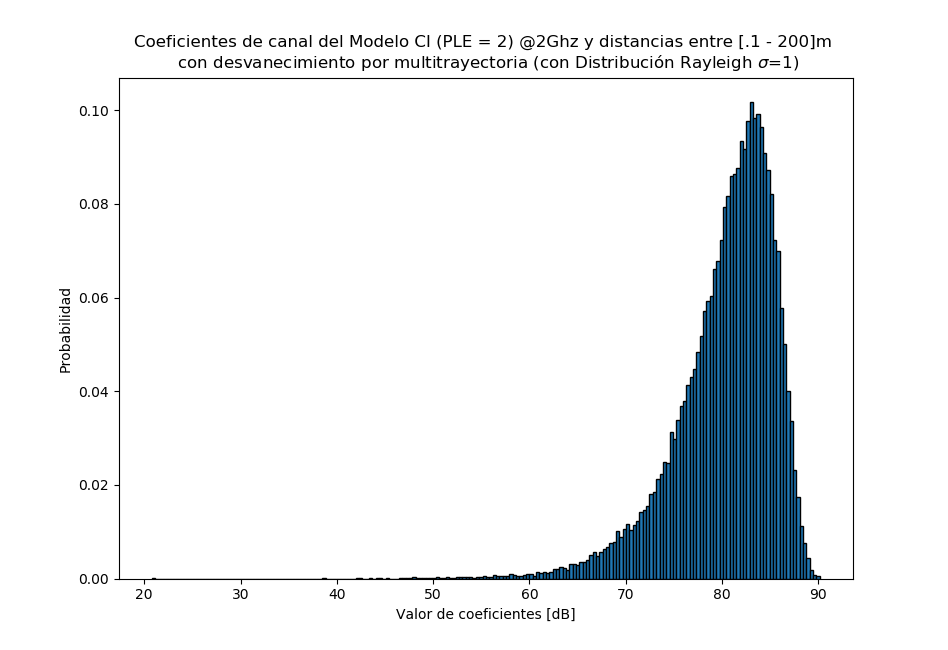
\includegraphics[scale=.55]{Figures/CoeficientesCanalCI.png}
    \decoRule
    \caption[Ganancias de Canal Modelo CI]{Ganancias de Canal Modelo CI}
    \label{fig:GananciasCI_C6}
\end{figure}

\hfill

\break
%----------------------------------------------------------------------------------------
%	SECTION 
%----------------------------------------------------------------------------------------

\section{Esquema de acceso múltiple al medio no ortogonal, basado en potencia (PD-NOMA)}

De acuerdo con el modelo de sistema (sección~\ref{}), se propuso implementar un esquema de acceso múltiple no ortogonal (NOMA), con base en \parencite{Shahini2019}, los autores desarrollaron un esquema NOMA basado en NB-IoT por medio de un agrupamiento óptimo de los usuarios y una optimización en la asignación de recursos, de acuerdo con la maximización de la tasa de transmisión total de subida de los dispositivos MTC.\newline

\subsection{Algoritmo de Agrupación de dispositivos uRLLC  y mMTC}

Se implementó el algoritmo de agrupamiento NOMA para los dispositivos mMTC y uRLLC descrito en \parencite{Shahini2019}[\textit{véase Algorithm \ref{A1}}], este algoritmo realiza un ordenamiento conveniente con respecto al uso de la Cancelación Sucesiva de Interferencia (SIC), es decir, se ordenan los dispositivos URLLC y mMTC de acuerdo con su ganancia de canal promedio dentro de los diferentes grupos NOMA para que puedan compartir el mismo recurso espectral (subportadora) asignado a cada grupo[\textit{véase Figura~\ref{fig:NOMAgrupoexample}}]. El Algoritmo da prioridad a los dispositivos uRLLC para que obtengan los rangos más bajos. \newline

Por lo tanto, un mensaje combinado de los dispositivos mMTC y uRLLC con ruido aditivo es recibido en la BS, la BS emplea la recepción SIC de acuerdo en cómo son ordenados los dispositivos. \newline

La recepción SIC decodifica primero el mensaje del dispositivo con el rango más bajo, por consiguiente los usuarios con los rangos siguientes (o más altos) le introducen interferencia y a su vez el usuario con el rango más alto no experimenta interferencia de ninguna señal.\newline

Es importante notar que los dispositivos uRLLC tienen requerimientos de tasas de datos más altos, por lo tanto, su potencia de transmisión será mayor que la de los dispositivos mMTC. Es por esto que en cada grupo los dispositivos uRLLC tendrán los rangos más bajos y los dispositivos mMTC los más altos. De hecho, el decodificador SIC en la BS comienza a decodificar con URLLC y, en consecuencia, los dispositivos mMTC no se ven afectados por la alta interferencia de los URLLC [véase Figura NOMAgrupoexample].\newline




\begin{figure}[th]
    \centering
    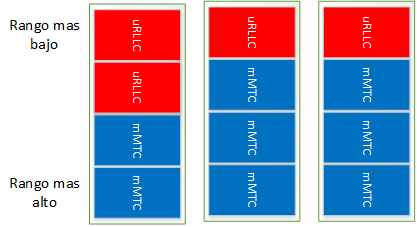
\includegraphics[scale=1]{Figures/EjemploNOMAclusters}
    \decoRule
    \caption[Ejemplo ilustrativo del ordenamiento de usuarios en los grupos NOMA]{Ejemplo ilustrativo del ordenamiento de 4 usuarios uRLLC y 8 usuarios mMTC en 3 grupos NOMA}
    \label{fig:NOMAgrupoexample}
\end{figure}





%%%%%%%%%%%%%%%%%%%%%%%%%%%%%%%%%%%%%%%%%%%%%%%%%%%%%%%%       EJEMPLO DE ALGORITMO EN LaTeX       %%%%%%%%%%%%%%%%%%%%%%%%%%%%%%%%%%%%%%%%%%%%%%%%%%%%%%%%%%%%%
Definición de variables de los algoritmos 1 y 2:\newline

\begin{itemize}
    \item U: Lista de dispositivos uRLLC
    \item M: Lista de dispositivoss mMTC
    \item S: Lista de Subportadoras s
    \item C: Lista de Grupos NOMA
    \item $R_{m}^{th}:$ Tasa objetivo del enésimo dispositivo m mMTC 
    \item $R_{u}^{th}:$ Tasa objetivo del enésimo dispositivo u uRLLC
    \item $P_{m}^{max}:$ Potencia máxima del enésimo dispositivo m mMTC 
    \item $P_{u}^{max}:$ Potencia máxima del enésimo dispositivo u uRLLC (i.e. 23dBm)
    \item $P_{m}^{s}:$ Potencia del enésimo dispositivo m mMTC 
    \item $P_{u}^{s}:$ Potencia del enésimo dispositivo u uRLLC 
    \item $h_{m}^{s}:$ Ganancia de canal del enésimo dispositivo m mMTC sobre la portadora s
    \item $h_{u}^{s}:$ Ganancia de canal del enésimo dispositivo u uRLLC sobre la portadora s
    \item ${\hat S}$: Lista de subportadoras asignadas
    \item $S_{a}^{c}$: Lista de subportadoras asignadas al enésimo cluster
    \item ${C_{ns}}$: Lista de cluster aún no asignados
\end{itemize}


\makeatletter
% Reinsert missing \algbackskip
\def\algbackskip{\hskip-\ALG@thistlm}
\makeatother

\begin{algorithm}
    \caption{Algoritmo de agrupamiento de dispositivos uRLLC y mMTC para NOMA}\label{A1}
    \hspace*{\algorithmicindent} \textbf{Entrada} $U, M, S, C, h_{m}^{s} , \ and \ h_{u}^{s} ,\forall m \in \mathcal {M} , \forall u \in \mathcal {U} , \forall s \in \mathcal {S}$  \\
    \hspace*{\algorithmicindent} \textbf{Salida} Lista de Clusters (C) con agrupamiento de dispositivos 
    \begin{algorithmic}[1]
    \Procedure{Agrupación de dispositivos uRLLC}{}\\
    Cálculo de la ganancia de canal promedio del enésimo dispositivo u\\
    ${\tilde h_{u}} =\sum \nolimits _{s \in \mathcal {S}} {h_{u}^{s}}{/_{|S|}}$\\
    Se ordenan descendentemente las ganancias de canal promedio de cada dispositivo u, i.e. $\forall u \in \mathcal {U} : {\tilde h_{1}} \geq {\tilde h_{2}} \geq \cdots \geq {\tilde h_{U}}$ 
    \For{\textbf{each} u in U}
        \If {$|U|<|C|$} 
        \State Asignar uRLLC al rango mas bajo (k=1)
        \Else
        \State Asignar uRLLC al siguiente rango (k=2) [Solo se podrán asignar hasta un segundo rango]
        \EndIf
    \EndFor
    \State Encontrar ${\tilde k}$, rango y grupo en el que se quedó la última asignación uRLLC
    \EndProcedure
    \Procedure{Agrupación de dispositivos mMTC}{${\tilde k}$}\\
    Cálculo de la ganancia de canal promedio del enésimo dispositivo u\\
    ${\tilde h_{m}} =\sum \nolimits _{s \in \mathcal {S}} {h_{m}^{s}}{/_{|S|}}$\\
    Se ordenan descendentemente las ganancias de canal promedio de cada dispositivo u, i.e. $\forall m \in \mathcal {M} : {\tilde h_{1}} \geq {\tilde h_{2}} \geq \cdots \geq {\tilde h_{M}}$ 
    \For{\textbf{each} m in M}
        \If {$|M|<|C|$} 
        \State Asignar mMTC al rango ${\tilde k}$
        \Else
        \State Asignar mMTC a los siguientes rangos \ldots
        \EndIf
    \EndFor
    \EndProcedure
    \end{algorithmic}
\end{algorithm}


\subsection{Algoritmo de Asignacion de Subportadoras}


Este algoritmo garantiza una óptima asignación de portadoras (S), de acuerdo con la maximización de la tasa total de transmisión, para los grupos NOMA. En \parencite{Shahini2019} se plantea la metodología para la asignación de subportadoras a los grupos NOMA. \newline

Cabe destacar que en \parencite{Shahini2019}, el modelo de sistema no es implementado hacia una banda de frecuencias en específico, las ganancias de las subportadoras son estadíticas por el uso de un desvanecimiento tipo Rayleigh dentro de su simulación.\newline

En nuestro caso como se ocupa un modelo de canal que depende de la frecuencia, se tuvo que escoger un PRB de 180 KHz, con un conjunto de subportadoras fijadas en una banda LTE, se escogió la banda de 2GHz, esto por el hecho de que LTE se implementa en bandas de microondas. \newline

Para cada subportadora, el mejor grupo (c*) es el que maximiza el rendimiento total, [\textit{véase Algorithm \ref{A2}}]. Luego, por consecuencia, las velocidades de datos de los dispositivos mMTC y URLLC y sus potencias de transmisión se actualizan. Durante el proceso de asignación de subportadoras, los clústeres asignados se excluyen del conjunto de Cns. \newline

El algoritmo asigna iterativamente las subportadoras disponibles una por una. Dado que cada dispositivo MTC divide por igual su potencia de transmisión máxima entre todas las subportadoras asignados, las potencias de transmisión de los dispositivos MTC a través de las diferentes subportadoras no son óptimas utilizando el algoritmo planteado. \newline

La fase de asignación de recursos termina hasta que las 48 subportadoras se asignan a los 48 clústeres NOMA, esto del hecho que se adapta para una transmisión singletone. \newline



\begin{figure}[th]
    \centering
    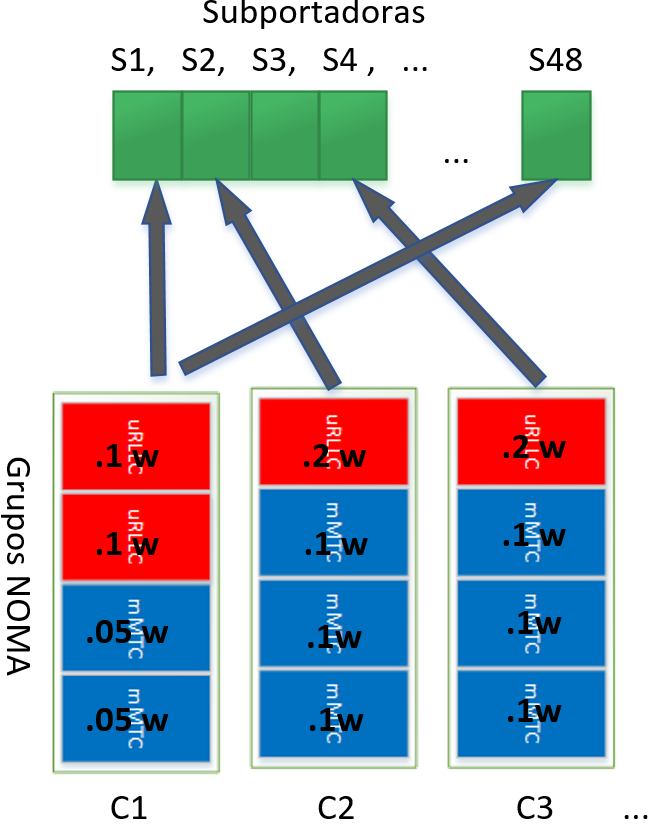
\includegraphics[scale=.5]{Figures/PD_NOMA_Cluster.png}
    \decoRule
    \caption[Ejemplo ilustrativo de la distribución de potencia para PD-NOMA en \textit{Multitone}]{Ejemplo ilustrativo de la distribución de potencia para PD-NOMA en \textit{Multitone}}
    \label{fig:NOMAgrupoexample}
\end{figure}


\begin{algorithm}
    \caption{Algoritmo de asignación de recursos para NOMA}\label{A2}
    \hspace*{\algorithmicindent} \textbf{Entrada} $U, M, S, C , R_{m}^{th} , R_{u}^{th} , P_{m}^{max} , P_{u}^{max} , h_{m}^{s} , \ and \ h_{u}^{s} ,\forall m \in \mathcal {M} , \forall u \in \mathcal {U} , \forall s \in \mathcal {S}$  \\
    \hspace*{\algorithmicindent} \textbf{Salida} Asignaciones de grupos con subportadoras (Asignación de todas las subportadoras [48, NB-IoT singletone]) 
    \begin{algorithmic}[1]
    \Procedure{Asignación de subportadoras}{}\\
    $Inicialización: $ \\${R_{u}} = 0 , {R_{m}} = 0 , p_{m}^{s}=P_{m}^{max} \ y \ p_{u}^{s}= P_{u}^{max} , \forall m \in \mathcal {M} , \forall u \in \mathcal {U} , \forall s \in \mathcal {S}.$ 
    ${\hat S} \leftarrow \emptyset,~~S_{a}^{c} \leftarrow \emptyset,~~{C_{ns}} \leftarrow \mathcal {C}$ 
    \While{$\mathcal{S} \ne \emptyset$}{}
    \BState \emph{Asignación de una subportadora a un grupo NOMA}:
        \For{\textbf{each} s in S}{
        \State Seleccionar al mejor cluster $c^{*}$ (el que maximiza el throughput):
        \State ${c^{*}} = \mathop {\arg \max }\limits _{c \in {C_{ns}}} \left ({{\sum \nolimits _{u \in \mathcal {U}} {R_{u} + \sum \nolimits _{m \in \mathcal {M}} {R_{m}} } } }\right) ;$ 
        \State donde: Ru \textit{(Ecuación \ref{eqn:Ru})} y Rm \textit{(Ecuación \ref{eqn:Rm})}, de acuerdo con \parencite{Shahini2019}
        \State $Asignar\ la\ subportadora\ s\ con\ c^{*} :$ 
        \State $Actualizar\ S_{a}^{c^{*}}\ \leftarrow S_{a}^{c^{*}} \cup \{ s\} , \hat S \leftarrow \hat S \cup \{ s\}$ 
        \State $Actualizar\ las\ tasas: {R_{u}} = {R_{u}} + {R_{u,s}} ,\ {R_{m}} = {R_{m}} + {R_{m,s}}$ 
        \State $Actualizar\ las\ potencias\ de\ los\ URLLC\ y\ mMTC\ de\ c^{*}\ individualmente:$ 
        \State $p_{m}^{s} = \frac {p_{m}^{s}}{{\left |{ {S_{a}^{c^{*}}} }\right | + 1}} ,\ p_{u}^{s} = \frac {p_{u}^{s}}{{\left |{ {S_{a}^{c^{*}}} }\right | + 1}} , \forall s \in \mathcal {S}$ 
        \If {$ S_{a}^{c^{*}} == 1$}{
        \State ${C_{ns}} \leftarrow {C_{ns}}\backslash \{{c^{*}}\}$ 
        \EndIf}
        \EndFor}
    \EndWhile
    \BState \emph{Asignación de subportadoras restantes}:
    \If {$ C_{ns} \ne \emptyset $} { 
        \For{\textbf{each} s in S}{
            \State $\mathcal {S} \leftarrow \mathcal {S}\backslash \hat S$ 
            \State ${c^{*}} = \mathop {\arg \max }\limits _{c \in {C}} \left ({{\sum \nolimits _{u \in \mathcal {U}} {R_{u} + \sum \nolimits _{m \in \mathcal {M}} {R_{m}} } } }\right)$ 
            \State $Actualizar\ S_{a}^{c^{*}} \leftarrow S_{a}^{c^{*}} \cup \{ s\}$ 
        \EndFor}
            \State $Actualizar\ p_{m}^{s} = \frac {p_{m}^{s}}{{\left |{ {S_{a}^{c^{*}}} }\right | + 1}} ,\ p_{u}^{s} = \frac {p_{u}^{s}}{{\left |{ {S_{a}^{c^{*}}} }\right | + 1}}$ 
    \EndIf}
    \EndProcedure
    \end{algorithmic}
\end{algorithm}



\begin{algorithm}
    \caption{Modo de Operacion \textit{Multitone}}\label{euclid}
    \hspace*{\algorithmicindent} \textbf{Entrada} NumeroDispositivos\\
    \hspace*{\algorithmicindent} \textbf{Output} NumeroGrupos
    \begin{algorithmic}[1]
    \Procedure{Ejemplo de procedimiento \textit{Multitone} con kmax=4}{}
    \If {$kmax ==4$} 
        \If {$NumeroDispositivos <= 48$} 
        \Return NumeroDispositivos
        \EndIf
        \If {$NumeroDispositivos > 48\ and\ NumeroDispositivos <=96$} 
        \Return NumeroDispositivos/2
        \EndIf
        \If {$NumeroDispositivos > 96\ and\ NumeroDispositivos <= 144 $} 
        \Return NumeroDispositivos/3
        \EndIf
        \If {$NumeroDispositivos > 144\ and\ NumeroDispositivos < 192$} 
        \Return NumeroDispositivos/4
        \EndIf
        \If {$NumeroDispositivos >= 192$} 
        \Return 48
        \EndIf
    \EndIf
    \EndProcedure
    \end{algorithmic}
    \end{algorithm}

\subsection{Escenario de Prueba de NOMA}

En este escenario de pruebas, evaluamos el rendimiento del sistema del esquema NB-IoT basado en NOMA propuesto en \parencite{Shahini2019}, el cual implementó dos Algoritmos uno para la formación de grupos y otro para la asignación de recursos. \newline

Consideraron una celda con un radio de 0.5 km donde las ubicaciones de los dispositivos mMTC y URLLC se generaron aleatoriamente (de manera uniforme) dentro de la celda. Además, consideraron un solo PRB con 48 subportadoras de 3.75 kHz para las transmisiones de enlace ascendente (UL) en un intervalo de tiempo (TTI). \newline

Modelaron las ganancias de canal de los dispositivos mMTC como $h_{s}^{m} = \gamma d^{ -\beta}_{ m, s}$ (de manera similar $h_{s}^{u}$ para URLLCs), donde $\gamma$ es un valor aleatorio generado por la PDF de Rayleigh, $d_{-\beta}^{m,s}$ representa la distancia entre el UE y la BS, y $\beta$ es el PLE el cual lo establecieron en $\beta = 3$ y $d$ varía entre 0.1 y 500 m. \newline

También, consideraron el ruido gaussiano blanco aditivo $(AWGN)$ con una densidad espectral de potencia de $-173 dBm / Hz$. Los presupuestos de potencia de transmisión máxima de todos los dispositivos URLLC y mMTC, $Pmax ^{u}$ y $Pmax ^{m}$ ($\forall m \in \mathcal {M} , \forall u \in \mathcal {U}$), se establecen en 23 dBm. Los umbrales de velocidad de datos de los dispositivos mMTC siguen una distribución uniforme, es decir, $R_{th}^{ m} = Uniforme (0.1, 2) kb / s$, $R_{th}^{u} = Uniforme (0.1, 20) kb / s$.\newline

Los autores en \parencite{Shahini2019} proponen la oportunidad de asignar más de una subportadora (\textit{multitone}) por grupo NOMA en transmisiones con anchos de banda UL de 3.75KHz para NB-IoT. Entonces, aunque aún no ha sido especificado la asignación de múltiples subportadoras por cluster en anchos de banda de 3.75KHz para NB-IoT, se tomó la propuesta de \parencite{Shahini2019} en este simulador. \newline

Cabe destacar que no necesariamente deben coincidir nuestros resultados con los del artículo ya que se tomaron algunas consideraciones diferentes a la de ellos. En la implementación del Algoritmo \ref{A2} se percató que los autores \parencite{Shahini2019} siempre buscan alcanzar la tasa objetivo de cada dispositivo uRLLC y mMTC en cada cluster haciendo la agregación de multiples subportadoras a cada clúster, el problema que surge con esto, es que muchas de las veces que se corría la simulación, la mayoría de las subportadoras se asignaban de entre 1 - 3 clusters esto porque parecía difícil cumplir con las tasas de todos los dispositivos en estos grupos, dejando a los otros grupos sin subportadora. La modificación que se implementó es que siempre se logre asignar una subportadora para cada grupo aunque sus dispositivos no alcancen su tasa objetivo, es decir se adoptó un número fijo de grupos NOMA igual a 48. \newline

Se intentó aplicar una transmisión \textit{multitone} de otro modo, analizemos el siguiente ejemplo: \newline

En un TTI, 50 dispositivos desean transmitir, en un modo \textit{singletone} se crearían siempre 48 grupos, entonces, 48 usuarios se agruparían en el primer rango de cada grupo y los otros dos restantes se agruparían en el segundo rango de los dos primeros grupos. En este caso no puede hacerse \textit{multitone} ya que las 48 subportadoras son ocupadas por cada grupo NOMA. \newline

Ahora bien, un modo \textit{multitone} se podría aplicar de la siguiente manera, si se consideran de igual manera 50 dispositivos queriendo transmitir, estos se pueden dividir en dos grupos de 25 dispositivos, es decir crear 25 grupos con su primer y segundo rangos completos, esto con la finalidad de que las 23 subportadoras restantes se agreguen en los grupos donde sus dispositivos aún no alcanzan su tasa objetivo, esto se implementó siguiendo la metodología del $Algorithm$ \ref{A3}. \newline

Al comparar los resultados entre \textit{multitone} y \textit{singletone} en la Figura XXX se puede que el desempeño de ambos es similar, solo un caso, y es cuando el número de dispositivos es menor al número de clusters, es decir, en un modo \textit{singletone}.\newline

\begin{figure}[th]
    \centering
    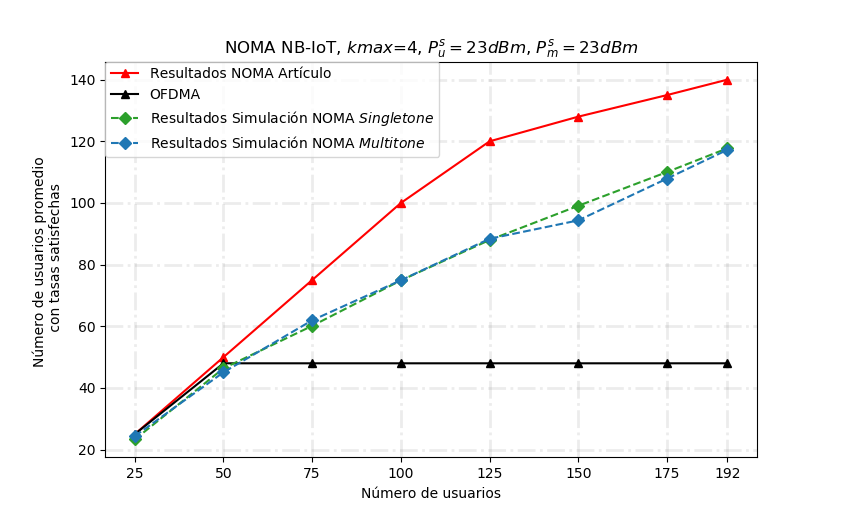
\includegraphics[scale=.7]{Figures/NOMA_results_comparation.png}
    \decoRule
    \caption[]{}
    \label{fig:ResultsNOMA}
\end{figure}

El impacto de la agregación de las subportadoras solo beneficia a aquellos dispositivos que tienen una buena condición de canal o que están en los últimos rangos (ya que experimentan menos interferencia). \newline

Se estudió de igual manera el impacto de \textit{multitone} con diferentes clases de potencia para los dispositivos MTC con $kmax = 4$ y su desempeño no resultó ser favorable. Igualmente, se evaluó el desempeño con diferentes tamaños de grupos. Por ese motivo esos resultados no se reportaron.\newline

Como se observa, no se logran satisfacer todos los requisitos de velocidad de datos de los dispositivos mMTC y URLLC pero si se incrementa significativamente la conectividad de usuarios en comparación con OFDMA donde solo se puede dar servicio a un usuario por subportadora, lo que son 48 usuarios.\newline


\begin{figure}[th]
    \centering
    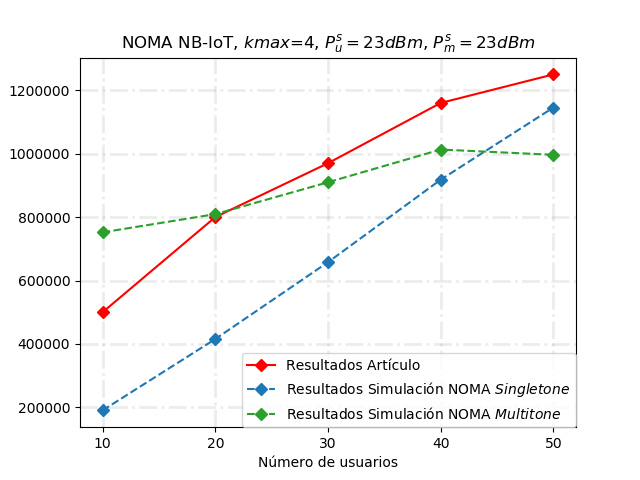
\includegraphics[scale=.7]{Figures/NOMA_sumrate.png}
    \decoRule
    \caption[]{}
    \label{fig:ResultsNOMA}
\end{figure}

\begin{figure}[th]
    \centering
    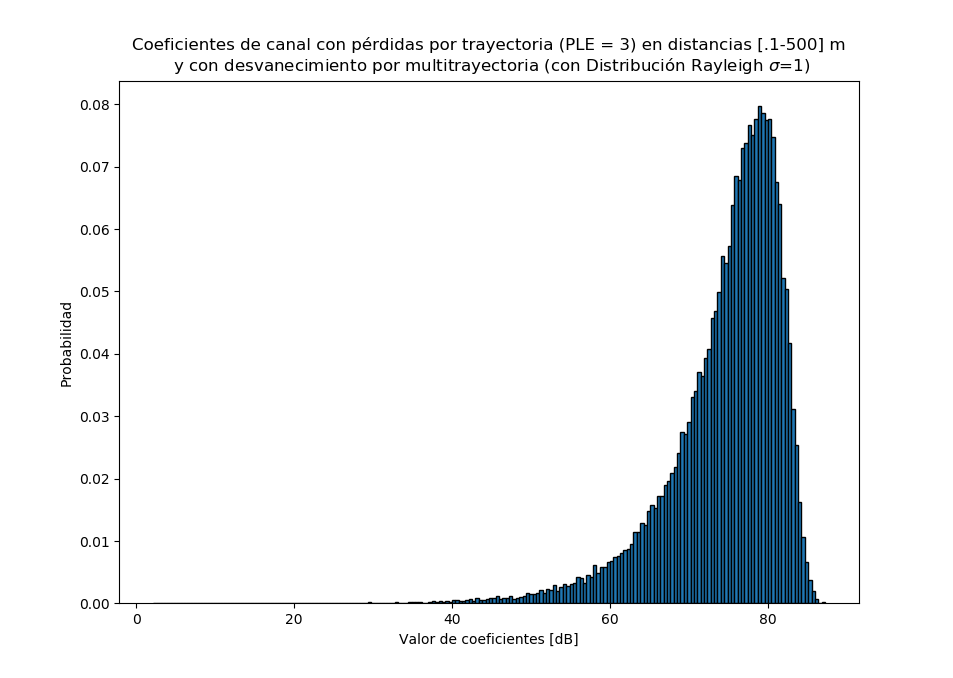
\includegraphics[scale=.7]{Figures/CoeficientesCanalShahini}
    \decoRule
    \caption[]{}
    \label{fig:CoeficientesCanalShahini}
\end{figure}





\hfill

\break

%----------------------------------------------------------------------------------------
%	SECTION 
%----------------------------------------------------------------------------------------

\section{Generación de Tráfico Fuente}
La generación de tráfico fuente requirió de un paradigma distinto al de eventos discretos, pues como se deja ver en el diagrama de la \textit{figura~\ref{fig:CMMPP_Algoritmo}}, un avance periódico en el tiempo es necesario para calcular las matrices de cambio de estado en los dispositivos y generar así el tráfico CMMPP, de esta manera el algoritmo de generación de tráfico fuente sigue un paradigma de simulación normalmente llamado \textit{time driven}. Adicional a este algoritmo se anexó la lógica para generar tráfico periódico en los dispositivos que así lo requirieran, teniendo así dos posibles modelos. Tal algoritmo corresponde al \textit{algoritmo \ref{A2}}. \newline

El programa Generador de Tráfico IoT se trata de la interconexión entre el algoritmo de distribución de usuarios, tratado en [6.1] y el de generación de tráfico fuente tratado en esta sección. A este programa se agrega una interfaz gráfica para facilitar la introducción de los parámetros que se consideran para generar el tráfico IoT y  se  describe más a detalle en la sección [6.6]. \newline

En las siguientes dos secciones se muestran los parámetros que fueron implementados para caracterizar el tráfico generado por los modelos CMMPP y Periódico. \newline
\subsection{Tráfico CMMPP}
La generación de tráfico CMMPP, sigue el diseño mostrado en la \textit{figura~\ref{fig:CMMPPpropuesta}} , para el cual cada dispositivo puede estar en estado de alarma o estado normal en un instante dado. El estado normal representa la operación habitual del dispositivo y a esta la caracteriza una tasa de arribos $ \lambda_{normal}$ que representa la cantidad promedio de paquetes por segundo que un dispositivo genera al estar en este estado. El estado de alarma por otra parte representa la detección de un evento o estado de interés especial para el dispositivo. Esta detección genera un único paquete de tamaño fijo detrás del cual el dispositivo volvería a su estado de operación habitual.\newline

El cambio de estado de normal  al estado de alarma requiere primeramente de un proceso en la simulación que se encargue de generar alarmas para cada tipo de dispositivo, este proceso se caracteriza por una tasa de arribo de alarmas $ \lambda_{alarma}$. Esta tasa representa la cantidad promedio de alarmas por segundo que ocurrirán en el área de la célula, además de este parámetro se necesita especificar la velocidad a la que las alarmas se transmiten desde su lugar de origen.\newline

El siguiente proceso que propicia un cambio de estado, es el cálculo de la matriz de cambio de estado $P_n\left[k\right]$ que se lleva a cabo en cada dispositivo. La ecuación \ref{eqn:Pn} utiliza la información de cuándo y donde se produjeron eventos de alarma, además de su velocidad de propagación para determinar el momento en el que la alarma llega al dispositivo. Adicionalmente es necesario un modelo que caracterice la propagación espacial. Los modelos implementados fueron los propuestos en [A] :\newline

\begin{equation}
\delta_n = e^{-\alpha.d_{n}}
\label{eqn:dn1}
\end{equation}

\begin{equation}
    \delta_n =
    \begin{cases}
        1  & \text{si $d_n < d_{th}$} \\
        \frac{1}{2}(1-sin\frac{\pi(d_n-W)}{2(W-d_{th})}) & \text{si $d_{th}< d_n < 2W-d_{th}$}\\
        0  & \text{si $d_n > 2W-d_{th}$}
    \end{cases}
    \label{eqn:dn2}
\end{equation}

El modelo que describe la \textit{ecuación~\ref{eqn:dn1}} se trata del \textit{decaying exponential} y está pensado para simular alarmas cuyo efecto en los dispositivos se espera siga un comportamiento exponencial. Los tipos de dispositivos que utilicen este modelo deberán especificar la constante $\alpha$ que caracteriza al modelo. Por otra parte la \textit{ecuación~\ref{eqn:dn2}} se trata de una \textit{raised-cosine window}, esta función es útil para modelar alarmas que se transmiten fuertemente por cierta distancia pero que después se detienen abrúptamente. Los tipos de dispositivos que utilicen este segundo modelo deberán especificar las constantes $d_{th}$ y $W$, donde $W$ es el ancho de la ventana y $d_{th}$ es la distancia de corte. En ambas ecuaciones $d_n$ es la distancia del dispositivo al origen de la alarma.\newline

Expuesto esto, los parámetros necesarios para la generación de tráfico con el modelo CMMPP, los cuales variarán según se decida para cada tipo de dispositivo, se encuentran en la \textit{tabla~\ref{tab:ParametrosTraficoCMMPP}}.\newline

\begin{table}
    \caption{Parámetros necesarios para generar tráfico CMMPP}
    \label{tab:ParametrosTraficoCMMPP}
    \centering
    \begin{tabular}{|m{6cm}|p{10cm}|} \\ 
    \textbf{Parámetro} & \textbf{Descripción} \\ 
    \textit{Tasa de nacimiento de paquetes $\lambda_{normal}$}  & \footnotesize{ Media de nacimiento de paquetes por segundo en cada dispositivo } \\ \hline 
    \textit{Tasa de nacimiento de alarmas $\lambda_{alarma}$}  & \footnotesize{ Media de nacimiento de alarmas } \\ \hline 
    \textit{Velocidad de propagación de alarmas}  & \footnotesize{ Velocidad a la que se propaga una alarma desde su posición de origen hacia todas direcciones. } \\ \hline 
    \textit{Modelo de propagación espacial de las alarmas} & \footnotesize{ Ya sea \textit{decaying exponential} o \textit{raised-cosine window}. } \\ \hline 
    \textit{Constante 1 propagación espacial} & \footnotesize{ Si el modelo de propagación corresponde a \textit{decaying exponential}:
    se trata de la constante $\alpha$, factor de decaimiento.
    Si el modelo de propagación corresponde a \textit{raised-cosine window}:
    se trata de la constante $W$, ancho de la ventana. } \\ \hline 
    \textit{Constante 1 propagación espacial} & \footnotesize{ Si el modelo de propagación corresponde a \textit{decaying exponential}:
    esta constante no se utiliza.
    Si el modelo de propagación corresponde a \textit{raised-cosine window}:
    se trata de la constante $d_{th}$, distancia de corte. } \\ \hline 
    \end{tabular}
\end{table}

    Con lo que respecta al tamaño de los paquetes, aquellos generados a partir del estado de alarma son de 20 $bytes$ y los generados en el estado normal siguen una distribución de Pareto con $\alpha$ = 2.5, tamaño mínimo de 20 $bytes$ y máximo de $200$ bytes.\newline

\subsection{Tráfico Periódico}

La generación del tráfico periódico no requiere mas que de un parámetro, la frecuencia de nacimiento de paquetes $F_{nacimiento}$, que es inversa al periodo de nacimiento de estos mismos $T_{nacimiento}$. En la implementación además, el tiempo del primer nacimiento de cada dispositivo que siga este modelo se calcula siguiendo una distribución uniforme que genera un valor entre 0 y el periodo de nacimiento y a partir de ahí se genera un nuevo nacimiento una vez transcurrido un periodo $T_{nacimiento}$. De esta manera, la transmisión de paquetes desde distintos dispositivos del mismo tipo se encuentra distribuida uniformemente a lo largo de un periodo.\newline

La \textit{tabla~\ref{tab:ParametrosTraficoPeriodico}} muestra el parámetro necesario para generar tráfico con el modelo periódico.\newline

\begin{table}
    \caption{Parámetros necesarios para generar tráfico Periódico}
    \label{tab:ParametrosTraficoPeriodico}
    \centering
    \begin{tabular}{|m{6cm}|p{10cm}|} \\ 
    \textbf{Parámetro} & \textbf{Descripción} \\ 
    \textit{Frecuencia de nacimiento de paquetes $F_{nacimiento}$}  & \footnotesize{ Cantidad de paquetes que genera un dispositivo por segundo, inversa al periodo entre dos nacimientos $T_{nacimiento}$. } \\ \hline 
 
    \end{tabular}
\end{table}

\subsection{Algoritmo de generación de tráfico fuente}

El programa de generación de tráfico fuente, implementa la generación de tráfico CMMPP y periódico según lo requiera cada tipo de dispositivo. El tráfico en cada tipo de dispositivo está caracterizado por los parámetros de entrada descritos en las \textit{tablas \ref{tab:ParametrosTraficoCMMPP} y \ref{tab:ParametrosTraficoPeriodico}}. Esta caracterización es compartida entre todos los dispositivos del mismo tipo, pero será diferente con dispositivos de otros tipos, según se seleccionen los parámetros.\newline

El \textit{algoritmo~\ref{generacionTrafico}} describe el proceso seguido por el programa de generación de tráfico.

\begin{algorithm}
    \caption{Generación de tráfico fuente}
    \label{generacionTrafico}
    \hspace*{\algorithmicindent} \textbf{Entrada} NumeroDispositivos\\
    \hspace*{\algorithmicindent} \textbf{Output} NumeroGrupos
    \begin{algorithmic}[1]
    \Procedure{Ejemplo de procedimiento \textit{Multitone} con kmax=4}{}
    \If {$kmax ==4$} 
        \If {$NumeroDispositivos <= 48$} 
        \Return NumeroDispositivos
        \EndIf
        \If {$NumeroDispositivos > 48\ and\ NumeroDispositivos <=96$} 
        \Return NumeroDispositivos/2
        \EndIf
        \If {$NumeroDispositivos > 96\ and\ NumeroDispositivos <= 144 $} 
        \Return NumeroDispositivos/3
        \EndIf
        \If {$NumeroDispositivos > 144\ and\ NumeroDispositivos < 192$} 
        \Return NumeroDispositivos/4
        \EndIf
        \If {$NumeroDispositivos >= 192$} 
        \Return 48
        \EndIf
    \EndIf
    \EndProcedure
    \end{algorithmic}
\end{algorithm}

El \textit{algoritmo~\ref{generacionTrafico}} se programó en python 3.6 para realizar el escenario de pruebas y hacer inmediata su reutilización en el programa Generador de tráfico IoT. Los parámetros utilizados en el escenario de pruebas y sus resultados se encuentran en la siguiente sección.\newline

\subsection{Escenario de Prueba para la Generación de Tráfico}

El escenario de pruebas para el algoritmo de generación de tráfico considera los parámetros presentados en las \textit{tablas~\ref{tab:paramPruebaTrafico} y \ref{tab:paramPruebaTrafico}}.  En la primera tabla se encuentran los parámetros que caracterizan el tráfico de los 7 distintos servicios seleccionados en la sección de diseño. Estos parámetros fueron determinados a partir de la \textit{tabla~\ref{tab:AppsSimulacion}}. Los demás parámetros necesarios para la simulación se encuentran en la segunda tabla, y corresponden al Tiempo de corte de la simulación y al diferencial $\Delta T$. Este diferencial corresponde al avance de tiempo que tiene la simulación en cada ciclo. Los valores se seleccionaron como $3600$ y $1$ segundos respectivamente, debido a que las tasas de nacimiento de paquete y de alarma se encuentran a lo mas en el orden unas cuantas por minuto, de manera que no hay necesidad en tener una definición mayor a 1 segundo. Algunas tasas de nacimiento de paquetes y alarmas se encuentran en el orden de unas cuantas por hora como es el caso de los dispositivos de detección de terremotos, razón por la cual se decidió realizar la simulación a lo largo de 3600 segundos.\newline

\begin{table}
    \caption{Parámetros para el escenario de pruebas de tráfico}
    \label{tab:paramPruebaTrafico}
    \centering
    \begin{tabular}{|m{16cm}|p{20cm}|} \\ 
        \textbf{Tipo:} Control de Iluminación\\ \textbf{Cantidad de dispositivos:} 1000 \\ \textbf{Modelo de tráfico:} CMMPP \\ \textbf{Tasa/Frecuencia de nacimiento de paquetes:} 0.000556  $paquetes/seg$. \\ \textbf{Tasa de nacimiento de alarmas:} 0.002778 $alarmas/seg$. \\ \textbf{Velocidad de alarma:} 500 $metros/seg$. \\ \textbf{Modelo de propagación espacial:} \textit{Raised-cosine window} \\ \textbf{$W$:} 200 \\ \textbf{$d_{th}$:} 100 \\ \hline
        \textbf{Tipo:} Monitoreo del consumo de agua y electricidad \\ \textbf{Cantidad de dispositivos:} 500 \\ \textbf{Modelo de tráfico:} Periódico \\ \textbf{Tasa/Frecuencia de nacimiento de paquetes:} 0.001667  $paquetes/seg$. \\ \hline
        \textbf{Tipo:} Detección de terremotos\\ \textbf{Cantidad de dispositivos:} 500 \\ \textbf{Modelo de tráfico:} CMMPP \\ \textbf{Tasa/Frecuencia de nacimiento de paquetes:} 0.000278  $paquetes/seg$. \\ \textbf{Tasa de nacimiento de alarmas:} 0.002778 $alarmas/seg$. \\ \textbf{Velocidad de alarma:} 3000 $metros/seg$. \\ \textbf{Modelo de propagación espacial:} \textit{Decaying exponential} \\ \textbf{$\alpha$:} 0.4 \\ \hline
        \textbf{Tipo:} Monitoreo de contaminación del aire\\ \textbf{Cantidad de dispositivos:} 500 \\ \textbf{Modelo de tráfico:} Periódico \\ \textbf{Tasa/Frecuencia de nacimiento de paquetes:} 0.001111  $paquetes/seg$. \\ \hline
        \textbf{Tipo:} Control dinámico de semáforos\\ \textbf{Cantidad de dispositivos:} 1000 \\ \textbf{Modelo de tráfico:} Periódico \\ \textbf{Tasa/Frecuencia de nacimiento de paquetes:} 0.016667  $paquetes/seg$. \\ \hline
        \textbf{Tipo:} Otros dispositivos mMTC\\ \textbf{Cantidad de dispositivos:} 3000 \\ \textbf{Modelo de tráfico:} CMMPP \\ \textbf{Tasa/Frecuencia de nacimiento de paquetes:} 0.016667  $paquetes/seg$. \\ \textbf{Tasa de nacimiento de alarmas:} 0.033333 $alarmas/seg$. \\ \textbf{Velocidad de alarma:} 500 $metros/seg$. \\ \textbf{Modelo de propagación espacial:} \textit{Decaying exponential} \\ \textbf{$\alpha$:} 0.007  \\ \hline
        
    \end{tabular}
\end{table}

\begin{table}
    \caption{Parámetros para el escenario de pruebas de tráfico}
    \label{tab:paramPruebaTrafico2}
    \centering
    \begin{tabular}{|m{16cm}|p{20cm}|} \\ 
        \textbf{Tipo:} Dispositivos URLLC \\ \textbf{Cantidad de dispositivos:} 1000 \\ \textbf{Modelo de tráfico:} CMMPP \\ \textbf{Tasa/Frecuencia de nacimiento de paquetes:} 0.016667  $paquetes/seg$. \\ \textbf{Tasa de nacimiento de alarmas:} 0.033333 $alarmas/seg$. \\ \textbf{Velocidad de alarma:} 500 $metros/seg$. \\ \textbf{Modelo de propagación espacial:} \textit{Decaying exponential} \\ \textbf{$\alpha$:} 0.007  \\ \hline
        \textbf{Tiempo límite de simulación:} 3600 $segundos$ \\ \textbf{$\Delta T$:} 1 $segundo$ \\ \textbf{Radio de la célula:} 200 $metros$ \\ \hline
    \end{tabular}
\end{table}

Los resultados de la simulación se presentan en las siguientes gráficas las cuales muestran los histogramas de arribos para algunos servicios junto con de las distribuciones que estos siguen, además de algunos mapas de calor que muestran el comportamiento de la propagación espacial de las alarmas. \newline

\begin{figure}[th]
    \centering
    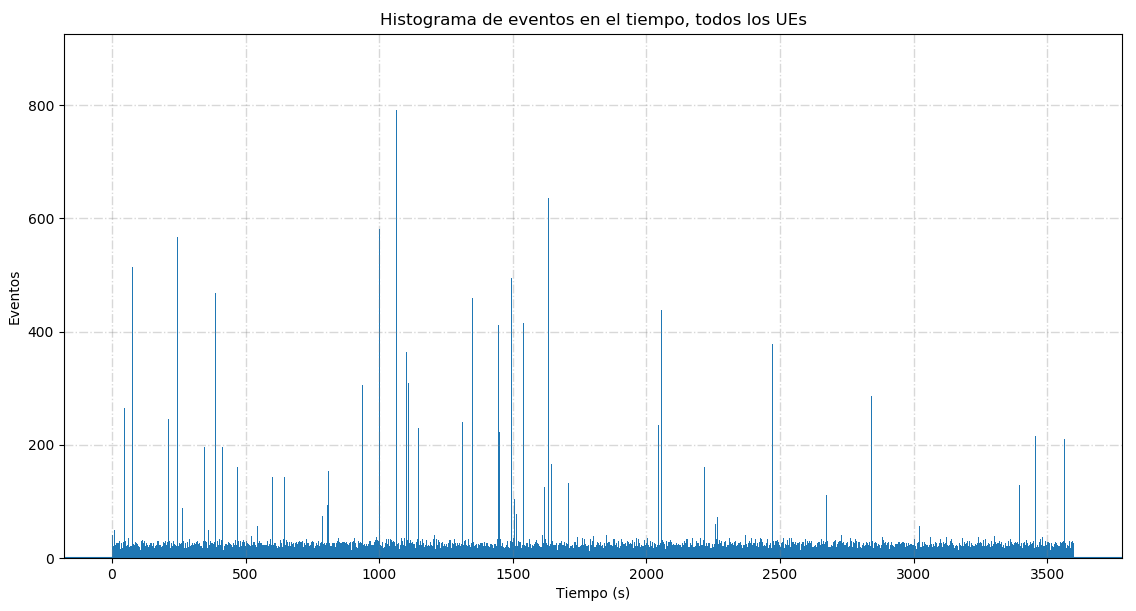
\includegraphics[scale=.4]{Figures/histoeventos.png}
    \decoRule
    \caption[Histograma de nacimientos de paquetes]{Histograma de nacimiento de paquetes}
    \label{fig:histoeventos}
\end{figure}

La \textit{imagen~\ref{fig:histoeventos}} muestra el histograma de nacimientos a lo largo de toda la simulación, el ancho de las barras es el mismo que $\Delta T$. En este histograma se contempla el tráfico generado por los 7 distintos servicios, de manera que es difícil extraer mucha información. A eso ayudan más las \textit{imagenes \ref{fig:histoeventos1} y \ref{fig:histoeventos2}}, las cuales se concentran en el tráfico de un sólo servicio, es decir de todos los dispositivos de un mismo tipo.\newline

\begin{figure}[th]
    \centering
    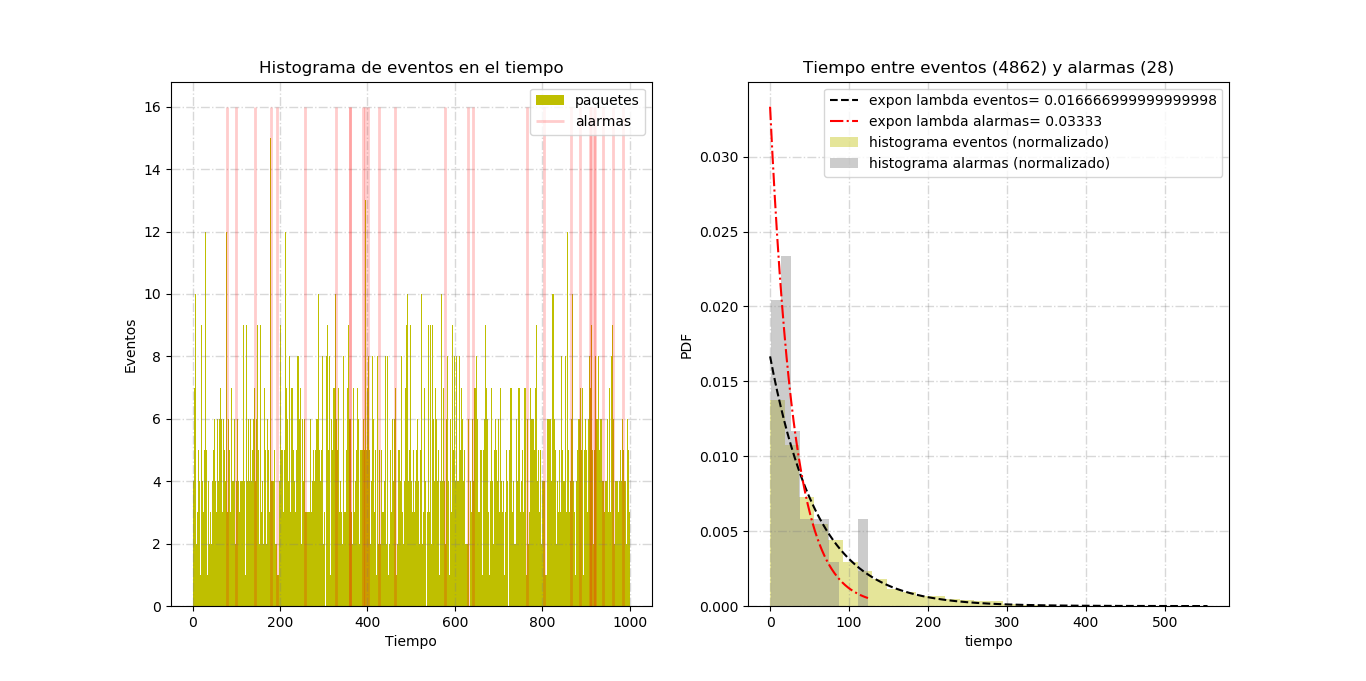
\includegraphics[scale=.4]{Figures/Otros_dispositivos_mMTC.png}
    \decoRule
    \caption[Otros dispositivos mMTC, Histograma de nacimientos y sus distribuciones]{Otros dispositivos mMTC, Histograma de nacimientos y sus distribuciones}
    \label{fig:histoeventos1}
\end{figure}

La \textit{imagen~\ref{fig:histoeventos1}} contiene a la izquierda el histograma de  nacimiento de paquetes junto con el nacimiento de las alarmas para los dispositivos  del tipo Otros dispositivos mMTC. Las gráficas a la derecha por otra parte son más fáciles de interpretar y se trata de la distribuciones que sigue el tiempo entre nacimiento de paquetes y de alarmas, las cuales podemos ver  siguen una distribución exponencial a la tasas establecidas como parámetros en la  \textit{tabla~\ref{tab:paramPruebaTrafico}}, justo como se esperaba.\newline

\begin{figure}[th]
    \centering
    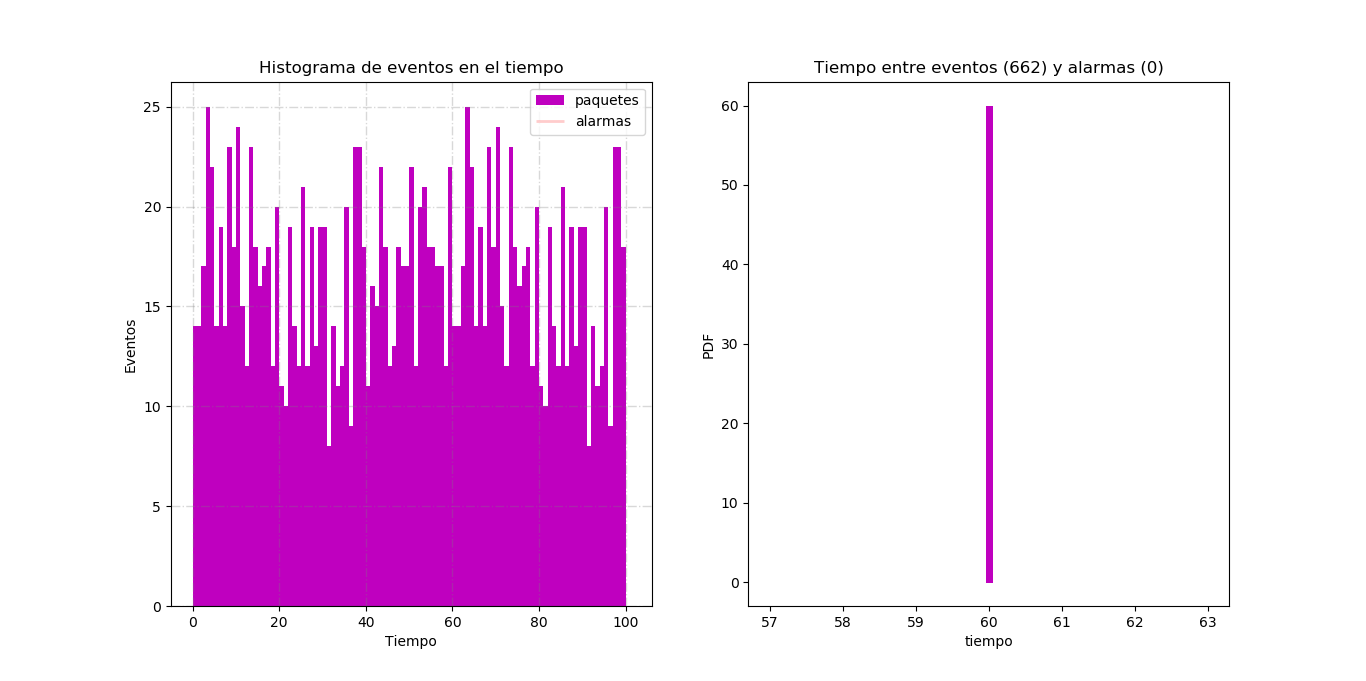
\includegraphics[scale=.4]{Figures/Semaforos_inteligentes.png}
    \decoRule
    \caption[Semáforos inteligentes, Histograma de nacimientos y sus distribuciones]{Semáforos inteligentes, Histograma de nacimientos y sus distribuciones}
    \label{fig:histoeventos2}
\end{figure}

La \textit{imagen~\ref{fig:histoeventos2}} es muy parecida a la \textit{imagen~\ref{fig:histoeventos1}} puesto que presenta las mismas gráficas, los histogramas a la izquierda y las distribuciones al derecha.  Pero en esta ocasión el servicio que observamos es el control de semáforos. Este servició genera  tráfico con el modelo periódico, razón por la cual el tiempo entre nacimiento de paquetes  es constante y no sigue una distribución exponencial.\newline

Finalmente en las \textit{imagenes \ref{fig:propagacion1} y \ref{fig:propagacion2}} se ven los mapas de calor producidos por una alarma que se transmite siguiendo el modelo \textit{Raised-cosine window} y \textit{Decaying exponential} respectivamente. Se puede notar cómo la propagación de la alarma siguiendo el modelo \textit{Raised-cosine window} tiene lugar de manera uniforme por dentro del círculo de radio dth  y con origen en su lugar de su nacimiento, para después desvanecerse y terminar abrúptamente para radios mayores al ancho de la ventana . Por otro lado la alarma que sigue el modelo de propagación exponencial se desvanece desde el origen y su efecto decae según crezca la distancia (de manera exponencial), pero no se detiene abrúptamente.\newline

\begin{figure}[th]
    \centering
    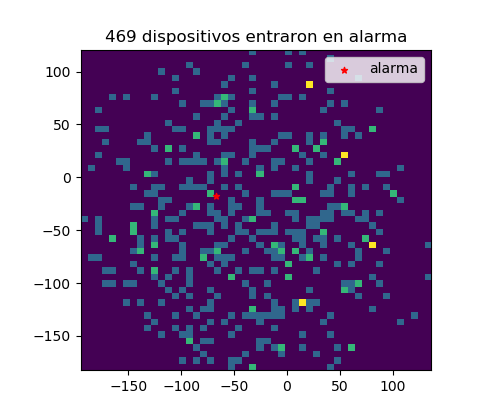
\includegraphics[scale=1]{Figures/UEs_de_tipo_Control_de_iluminacion_activados_por_una_alarma.png}
    \decoRule
    \caption[Propagación de alarma en dispositivos de control de iluminación]{Propagación de alarma en dispositivos de control de iluminación}
    \label{fig:propagacion1}
\end{figure}

\begin{figure}[th]
    \centering
    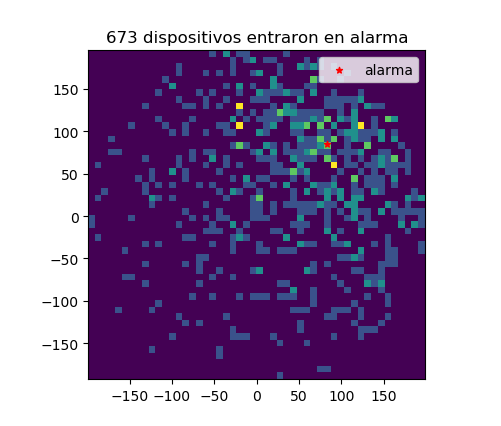
\includegraphics[scale=1]{Figures/UEs_de_tipo_Otros_dispositivos_mMTC_activados_por_una_alarma.png}
    \decoRule
    \caption[Propagación de alarma en otros dispositivos mMTC]{Propagación de alarma en otros dispositivos mMTC}
    \label{fig:propagacion2}
\end{figure}

Los resultados que presentan estas imágenes muestran que el algoritmo de generación de tráfico fuente está efectivamente generando arribos siguiendo los parámetros y modelos seleccionados, de manera que de aquí se procedió a su implementación en el programa \textbf{Generador de tráfico IoT} que se trata en la siguiente sección. \newline

\hfill

\break

%----------------------------------------------------------------------------------------
%	SECTION 
%----------------------------------------------------------------------------------------

\section{Interconexión de los 4 módulos del Simulador}

Los 4 módulos del sistema, cuya implementación se ha discutido en la primera parte de este capítulo son: el despliegue de los dispositivos, el modelo del canal, el esquema de acceso múltiple al medio y los modelos de tráfico IoT. La forma en la que se llevo acabo la interconexión de estos módulos se encuentra descrita en el diagrama de la \textit{imagen~\ref{fig:interconexion4}}. \newline

El simulador se encuentra entonces dividido en 2 programas, el \textbf{Generador de Tráfico IoT} y el \textbf{Simulador de eventos discretos}. La razón por la que se implemento esta arquitectura tiene que ver con los paradigmas que ambos programas siguen, ya que mientras el Generador de tráfico IoT tiene una rutina que realiza avances constantes en el tiempo, el Simulador de eventos discretos avanza en el tiempo apartir de los eventos evaluados. \newline

Ambos sistemas fueron programados en Python 3.6 y fueron implementados de manera modular. Es decir el programa Generador de Tráfico IoT es una herramienta funcional y modificable por sí sola para generar tráfico de tipo máquina con los modelos CMMPP y Periódico y con usuarios distribuidos a partir de un PPP. Los resultados de este programa podrían entonces ser utilizados en algúno otro, realizando los ajustes de interfaz necesarios. De la misma manera el Simulador de Eventos discretos que contiene el modelo del canal y el esquema de acceso múltiple al medio, podría procesar tráfico y usuarios generados y distribuidos en un programa distinto al presentado en este proyecto. Esta modularidad es posible en gran parte grácias a que la interfaz existente entre ambos programas es el uso de archivos .csv, los cuales son fáciles de generar y modificar.\newline

\begin{figure}[th]
    \centering
    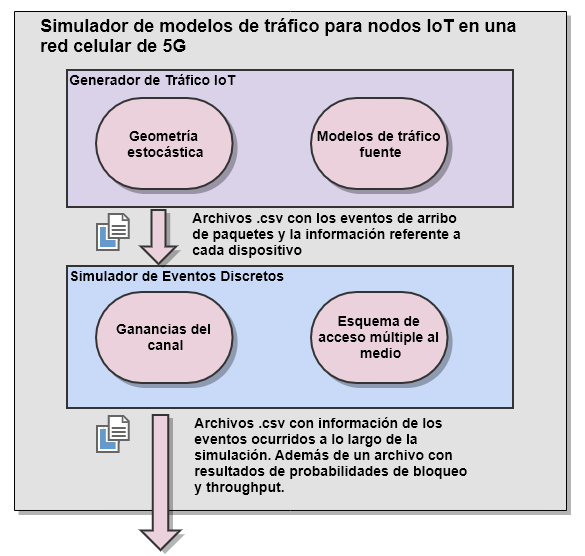
\includegraphics[scale=.7]{Figures/interconexion4modulos.png}
    \decoRule
    \caption[Interconexión de los 4 módulos en un simulador]{Interconexión de los 4 módulos en un simulador}
    \label{fig:interconexion4}
\end{figure}

En las siguientes secciones se aborda con más detalle la implementación de los dos programas que integran el simulador. \newline

\hfill

\break

%----------------------------------------------------------------------------------------
%	SECTION 
%----------------------------------------------------------------------------------------

\section{Generador de tráfico IoT}

    El Generador de tráfico IoT distribuye dispositivos IoT en una célula circular siguiendo un PPP, para después generar tráfico de estos dispositivos con los modelos CMMPP y Periódico. La rutina principal del programa sigue el paradigma \textit{time-driven}, puesto que realiza avances constantes en el tiempo. La salida del programa se da en forma de archivos .csv, de los cuales los dos más importantes son el archivo de dispositivos y el archivo de eventos. El archivo de dispositivos contiene información referente a cada uno de los dispositivos generados mientras que el archivo de eventos contiene la información del nacimientos de cada paquete.\newline

    La forma en que python se generaron y manipularon archivos .csv en python 3.6 fue con la librería $pandas$, la cual permite mapear listas a archivos .csv y viceversa. \newline

    Aunado a la funcionalidad principal del programa, se programó una interfaz de usuario para interactuar con el sistema e ingresar lo parámetros de la simulación. La interfaz de usuario se realizó con la librería $tkinter$. Esta interfaz se presenta con mayor detalle en la siguiente sección. \newline


\subsection{Interfaz de Usuario}

    La \textit{imagen~\ref{fig:GUITrafico}} es una captura de pantalla de la interfaz de usuario del Generador de Tráfico IoT. En el primer bloque arriba a la izquierda se encuentran parámetros referentes a la distribución de usuarios, como son el radio del área circular en la que se distribuirán y su modelo de distribución. Los siguientes 7 bloques sirven para introducir los parámetros de generación de tráfico para los 7 distintos servicios contemplados. Finalmente se debe indicar hasta abajo: el tiempo de corte de la simulación y el diferencial de tiempo entre ciclos antes de poder iniciar la rutina. El botón de cargar datos abajo a la derecha permite leer los parámetros de un archivo y desplegarlos en las casillas correspondientes, lo que permite guardar una configuración inicial y acelerar la introducción de valores. \newline

    
\begin{figure}[th]
    \centering
    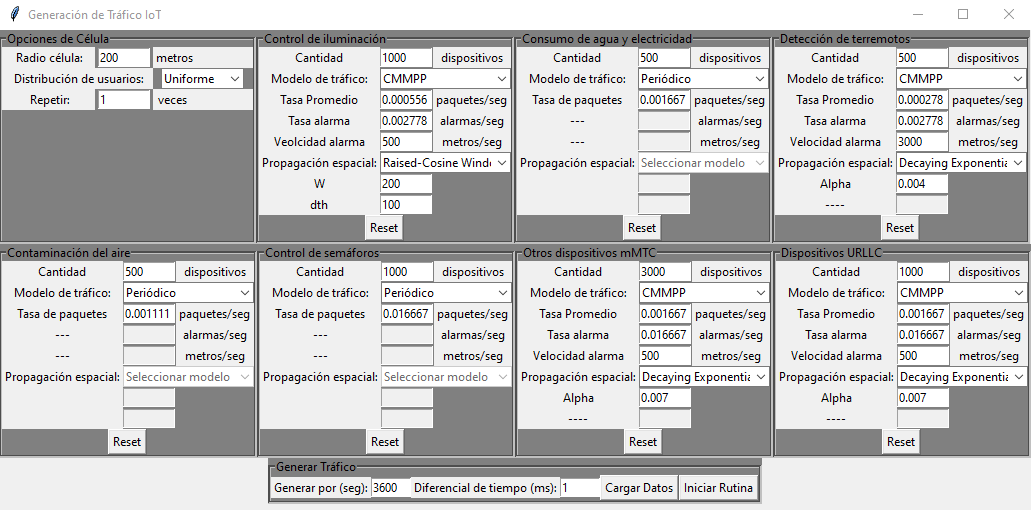
\includegraphics[scale=.6]{Figures/GUI.png}
    \decoRule
    \caption[Interfaz de Usuario, Generador de Tráfico IoT]{Interfaz de Usuario, Generador de Tráfico IoT}
    \label{fig:GUITrafico}
\end{figure}

Al terminar la rutina se generarán en la misma carpeta del programa 4 archivos .csv de los cuales 2 son utilizados en el \textbf{Simulador de eventos discretos}. Estos archivos son descritos con más detalle en la siguiente sección. \newline

\subsection{Archivos de Salida}

Los principales archivos que resultan de ejecutar cada rutina del Generador de Tráfico son el archivo de dispositivos y el archivo de eventos. En la \textit{imagen~\ref{fig:archivodispositivos}} se puede ver un ejemplo del primer archivo, en él se guarda: a qué tipo de dispositivo corresponde cada servicio y su posición en el plano. Estos datos son después utilizados en el Simulador de eventos discretos para instanciar nodos del tipo especificado en esa posición y poder adjudicarles sus nacimientos de paquetes. La \textit{imagen~\ref{fig:archivoeventos}} muestra un ejemplo de archivo de eventos, en el cual encontramos los nacimientos de paquetes a lo largo del tiempo de simulación. Desde tál archivo se podrá conocer el dispositivo que originó el paquete, su tamaño y si este surgió apartir de una alarma, todos estos datos importantes para que el simulador pueda procesar los eventos.  \newline

\begin{figure}[th]
    \centering
    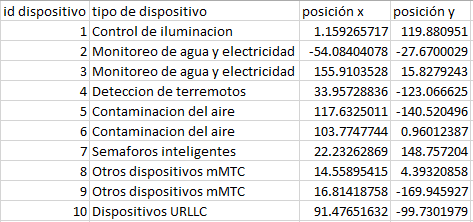
\includegraphics[scale=.7]{Figures/disparchivo.png}
    \decoRule
    \caption[Archivo de dispositivos]{Archivo de dispositivos}
    \label{fig:archivodispositivos}
\end{figure}

\begin{figure}[th]
    \centering
    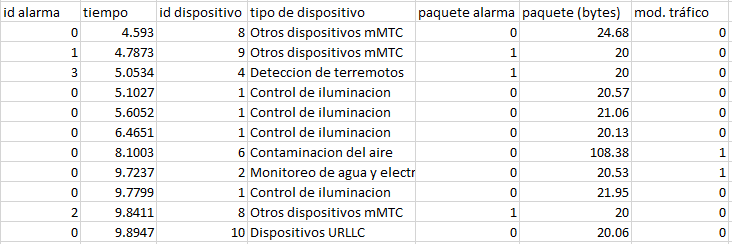
\includegraphics[scale=.7]{Figures/eventosarchivo.png}
    \decoRule
    \caption[Archivo de eventos]{Archivo de eventos}
    \label{fig:archivoeventos}
\end{figure}

Los últimos dos archivos resultados de cada rutina de este programa son el de configuración y el de alarmas. Pero estos no son utilizados por el Simulador de eventos, sino para generar gráficas de la distribución de usuarios y los modelos de tráfico y de distribución de alarmas.\newline

\hfill

\break


%----------------------------------------------------------------------------------------
%	SECTION 
%----------------------------------------------------------------------------------------

\section{Simulador de Eventos Discretos}

El Simulador de eventos discretos se trata del otro programa además del Generador de tráfico IoT que conforma al \textbf{Simulador de modelos de tráfico para nodos IoT en una red de 5G}. Fue también programado en python 3.6 y sigue el paradigma de eventos discretos. La funcionalidad básica del programa se puede observar en el diagrama de la \textit{imagen~\ref{fig:flowdes}}. En el diagrama se puede ver que cuando se toma el siguiente evento en la cola, este es procesado y es aquí donde la mayor parte de la lógica del simulador recide. En la siguiente sección se describen los distintos eventos y cómo son procesados.\newline

\begin{figure}[th]
    \centering
    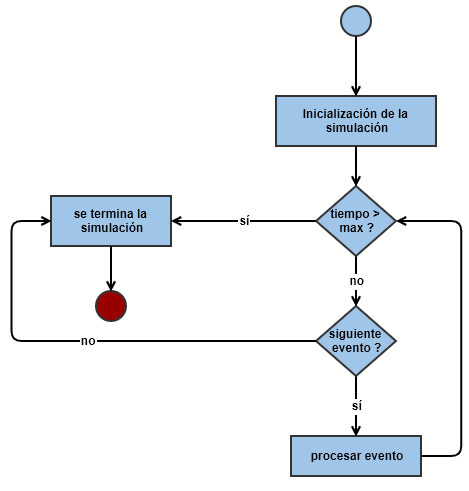
\includegraphics[scale=.7]{Figures/flowdes.png}
    \decoRule
    \caption[Simulación de eventos discretos]{Simulación de eventos discretos}
    \label{fig:flowdes}
\end{figure}

Para realizar la funcionalidad de eventos discretos en python se utilizó la librería $heapq$, la cual permite la utilización de \textit{heaps}, que son arboles binarios, para los cuales cada nodo padre tiene un valor menor o igual a cualquiera de sus hijos. De tal manera es posible mantener una lista que sigua esta estructura con el calendario de eventos (el arbol se ordena teniendo en cuenta el tiempo en el que ocurre el evento) y utilizar las funciones $heappush$ y $heappop$ para agregar nuevos eventos y removerlos del arbol respectivamente. Esta estructura asegura que el primer evento de la lista sea siempre el siguiente a ser evaluado y la librería representa una manera fácil de interactuar con la lista.\newline

A la salida del simulador, se tiene un archivo .csv con un historial de \textit{logs} correspondiente a los eventos que fueron procesados además de otro archivo con el resultado de las probabilidades de bloqueo por falta de cluster, el porcentaje de paquetes que fueron transmitidos a la tasa deseada y el \textit{throughput} del sistema. Los eventos que tienen lugar y son procesados por el sistema se presentan en la siguiente sección. \newline 

\subsection{Definición de eventos}

\begin{figure}[th]
    \centering
    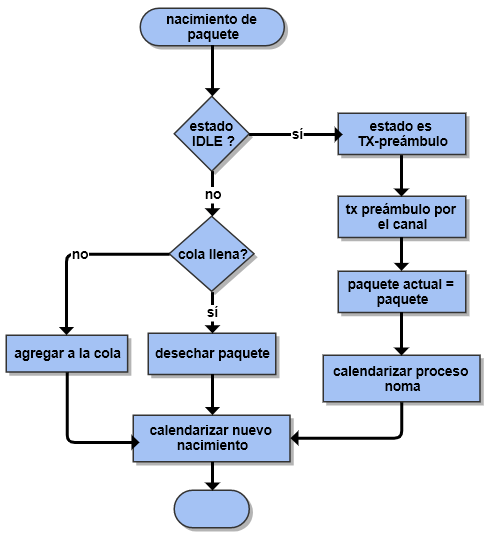
\includegraphics[scale=.7]{Figures/flownacimiento.png}
    \decoRule
    \caption[Procesamiento del evento: nacimiento de paquete]{Procesamiento del evento: nacimiento de paquete}
    \label{fig:flownacimiento}
\end{figure}

\begin{figure}[th]
    \centering
    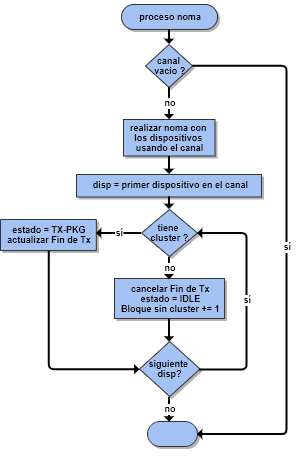
\includegraphics[scale=1]{Figures/flownoma.png}
    \decoRule
    \caption[Procesamiento del evento: proceso noma]{Procesamiento del evento: proceso noma}
    \label{fig:flownoma}
\end{figure}

\subsection{Descripción de los \textit{logs} de salida}

\subsection{Resultados a la salida del simulador}

\hfill

\break

%----------------------------------------------------------------------------------------
%	SECTION 
%----------------------------------------------------------------------------------------

\section{Optimización de tiempos de simulación}

La generación de distintas variables aleatorias y el uso de algoritmos de asignación de recursos nos mantuvo en la preocupación de que los tiempos de simulación probablemente llegarán a ser excesivamente largos, por tal se propuso utilizar una técnica de paralelismo en python. Favorablemente esto no sucedió como se esperaba, el tiempo máximo de espera para una simulación rondó los 20 minutos como máximo.\newline

De cualquier forma, la técnica de paralelización si se implementó pero solamente en la generación de resultados de NOMA para un TTI ya que en esta parte fue que se necesitaron obtener resultados promedio donde cada punto o muestra de los datos necesitaba simularse 1000 repeticiones para así obtener un promedio. En la Tabla~\ref{tab:} se observa la comparación de los tiempos de simulación e un caso normal (solamente 1 núcleo en uso) e implementando la paralelización (uso de todos los núcleos de la PC).\newline

[Cabe mencionar que esta simulación se montó en una PC con procesador Intel(R) Core(TM) i7-7700HQ CPU @2.80 GHz y 16 GB de Memoria RAM.]

